\documentclass[10pt, a4paper]{beamer}
\usetheme{Berkeley}
\usepackage{graphicx}
\usecolortheme{sidebartab}

\begin{document}
	\setbeamertemplate{sidebar left}{}
	\title{Progress Presentation-I}
	\subtitle{e-Yantra Summer Intership-2015 \\ \textbf{Controlling Firebird V using EEG sensor (Brainwave sensor)} }
	\author{\textbf{Members:}\\Omkar Rajendra Mohite\\Ashish Kumar Jain\\ 
	\textbf{Mentors:}\\Mehul Makwana\\Rutuja Ekatpure }
	\institute{IIT Bombay}
	\date{\today}
	%\addtobeamertemplate{sidebar left}{}{\includegraphics[scale = 0.3]{logowithtext.png}}
	\frame{\titlepage}

\setbeamertemplate{sidebar left}[sidebar theme]
\section{Overview of Project}
\begin{frame}{What is the project all about??...}
	\begin{itemize}
		\item \textbf{Name of the project:}\\Controlling Firebird V using EEG sensor (Brainwave sensor)
		\item \textbf{Objective:}\\The main objective of this project is to control the bot using brainwave sensor. This brainwave sensor analyses attention, meditation and various brain activities except human thoughts.
		\item \textbf{Deliverables:}\\\begin{enumerate}
			\item Tasks List
			\item Introduction to Brainwaves and sensor
			\item Various Task accomplished
			\item Challenges faced
			\item Future plans
		\end{enumerate}
	\end{itemize}
\end{frame}

\section{Overview of Task}
\begin{frame}{Overview of Task}
	\textbf{Tasks Accomplished:}
	\begin{enumerate}
	\item Understanding Brainwaves and about EEG sensor(Mindwave mobile headset)-----(2 days)
	\item Configuring Bluetooth module with sensor.-----(2 days)
	\item Analysing and Processing Brainwave values.-----(2 days)
	\item Interfacing Sensor to Firebird V via bluetooth.-----(3 days)
	\item LED Bargraph blinking based on Attention level-----(4 days)
\end{enumerate}
\textbf{Task Remaining:} 
\begin{enumerate}
	\item Controlling Firebird V motions using attention level and eye-blink.-----(5 days)
	\item Controlling wheel-chair using these techniques-----(5 days)
	\item Documentation-----(5 days)
\end{enumerate}
\end{frame}


\section{Introduction}
\begin{frame}{Introduction to Brainwaves}
	\begin{figure}[h]
		\caption{Five types of brainwaves measured from different sections of brain}
		\graphicspath{ {images/} }
		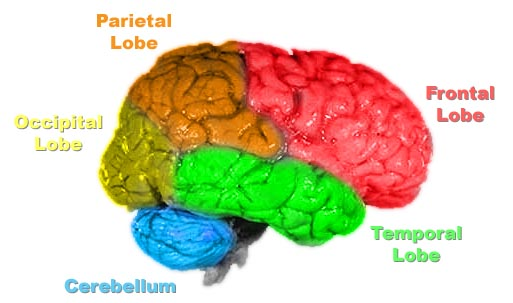
\includegraphics[width=5.5cm, height=3.2cm]{Brain-anatomy}
		\centering
	\end{figure}
	\begin{itemize}
		\item \textcolor{red}{Gamma waves} (24Hz to 100Hz from Center part of brain)
		\item \textcolor{red}{Beta waves} (12-30 Hz from cerebral cortex)
		\item \textcolor{red}{Alpha waves} (8-12 Hz from Occipital lobe)
		\item \textcolor{red}{Theta waves} (4-7 Hz from Hippocampus while dreaming)
		\item \textcolor{red}{Delta waves} (0-3 Hz from thalamus and cortex)
	\end{itemize}
\end{frame}

\section{Introduction}
\begin{frame}{What is EEG??...}
		\begin{itemize}
			\item EEG stands for \textbf{Electroencephalography}.
			\item Electroencephalography is a non-invasive method to record electrical activity of the brain along the scalp.
			\item This measures voltage fluctuations resulting from ionic current within the neurons of the brain.
		\end{itemize}
	
\end{frame}

\section{Task 1:Bluetooth Module}
\begin{frame}{Configuring bluetooth module(JY-MCU) using AT commands}	
	\begin{columns}[T]
		\begin{column}{.60\textwidth}
			\begin{block}{Connection of JY-MCU to USB to serial converter}
				\graphicspath{ {images/} }
				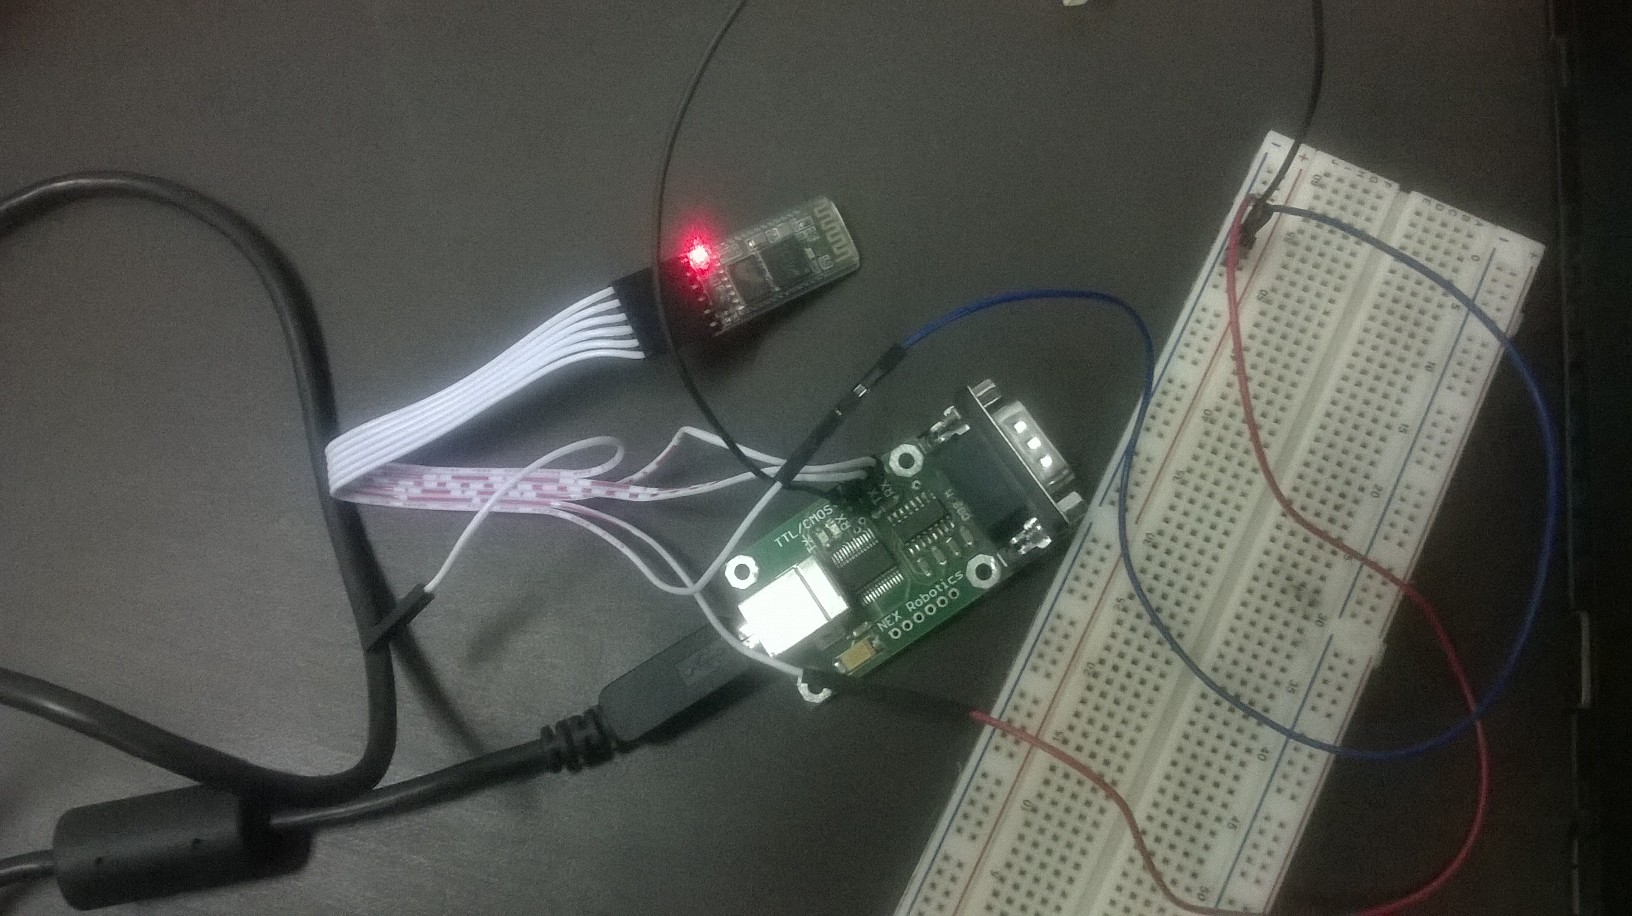
\includegraphics[width=4.8cm, height=3cm]{BT_Configure}
				\centering
				 \end{block}
				\end{column}
			\begin{column}{.40\textwidth}
				\begin{block}{Various AT commands for configuring module}
					\graphicspath{ {images/} }
					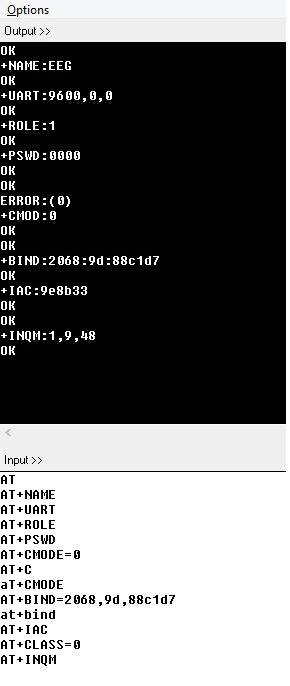
\includegraphics[width=2.8cm, height=5.2cm]{BT-AT_Configure}
					\centering
				\end{block}
			\end{column}
		\end{columns}
\end{frame}

\section{Task 2:Processing Brainwaves}
\begin{frame}{Processing Brainwaves using Arduino and Realterm}	
		\begin{columns}[T]
			\begin{column}{.45\textwidth}
				\begin{block}{Processing attention level data values using Arduino}
					\graphicspath{ {images/} }
					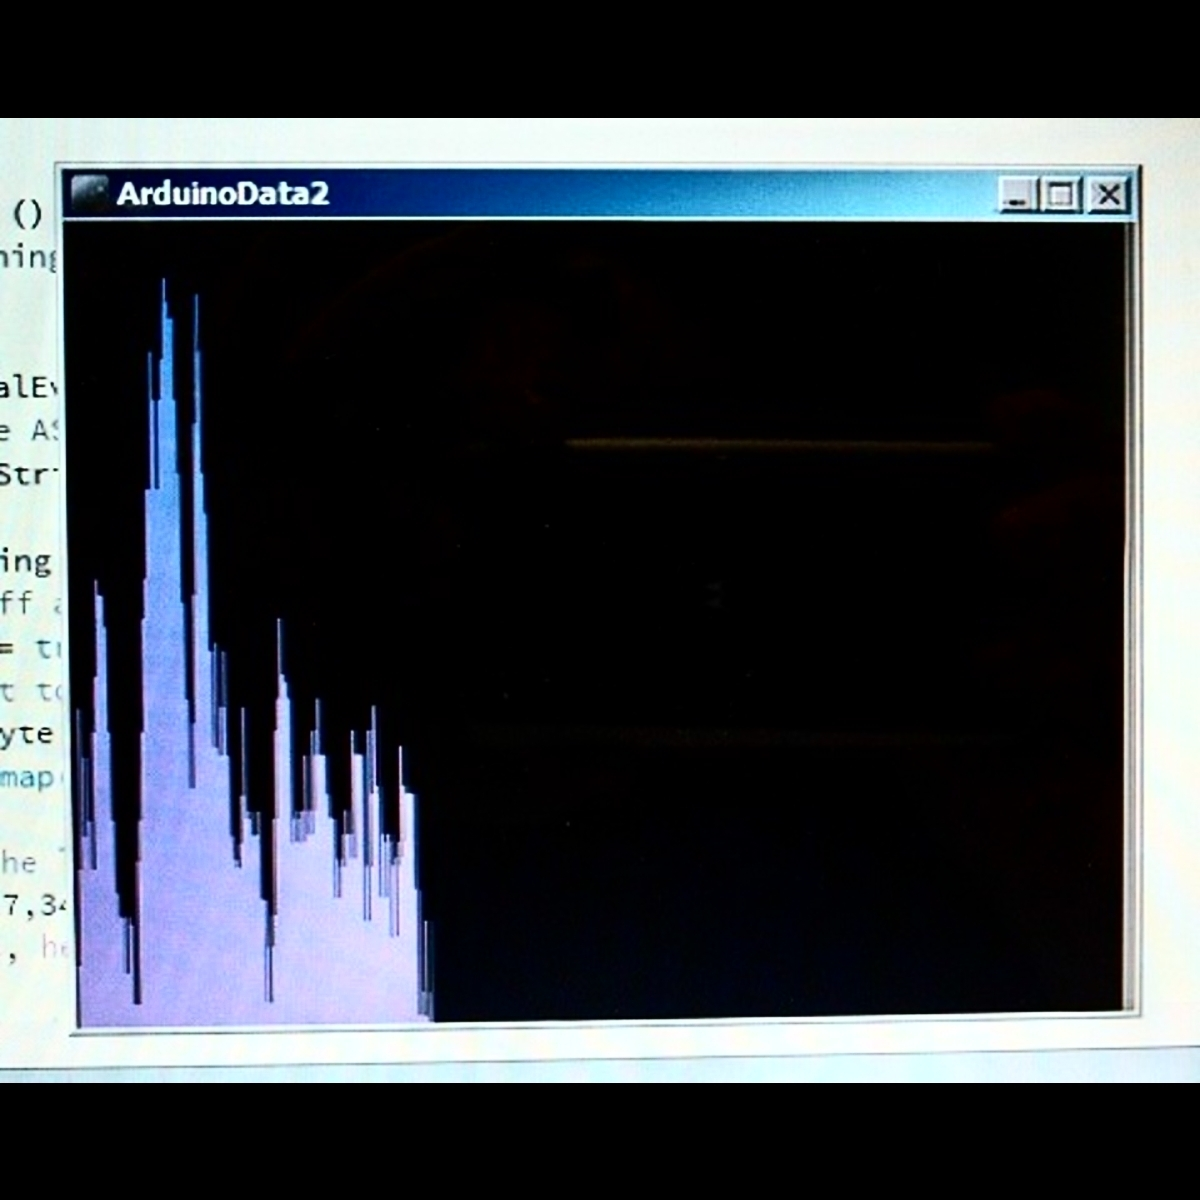
\includegraphics[width=5cm, height=5cm]{Arduino}
					\centering
				\end{block}
			\end{column}
			\begin{column}{.55\textwidth}
				\begin{block}{Analysing Data values using Realtern}
					\graphicspath{ {images/} }
					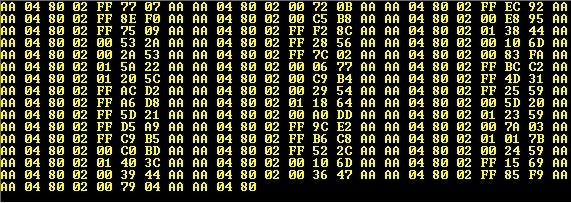
\includegraphics[width=5.5cm, height=2.4cm]{data_values1}
					\centering
				\end{block}
			\end{column}
		\end{columns}	
\end{frame}

\section{Task 3:Interfacing Sensor}
\begin{frame}{Interfacing Brainwave Sensor with Firebird V}
	\begin{itemize}
		\item Mindwave mobile sends data via bluetooth to firebird V bot.
		\item Bluetooth module(JY-MCU) is bound with Mindwave mobile using Unique ID.
		\item Initially Programmed the bot to just receive data values form sensor.  
	\begin{figure}[h]
		\caption{LED Indication of receiving data values from sensor.}
		\graphicspath{ {images/} }
		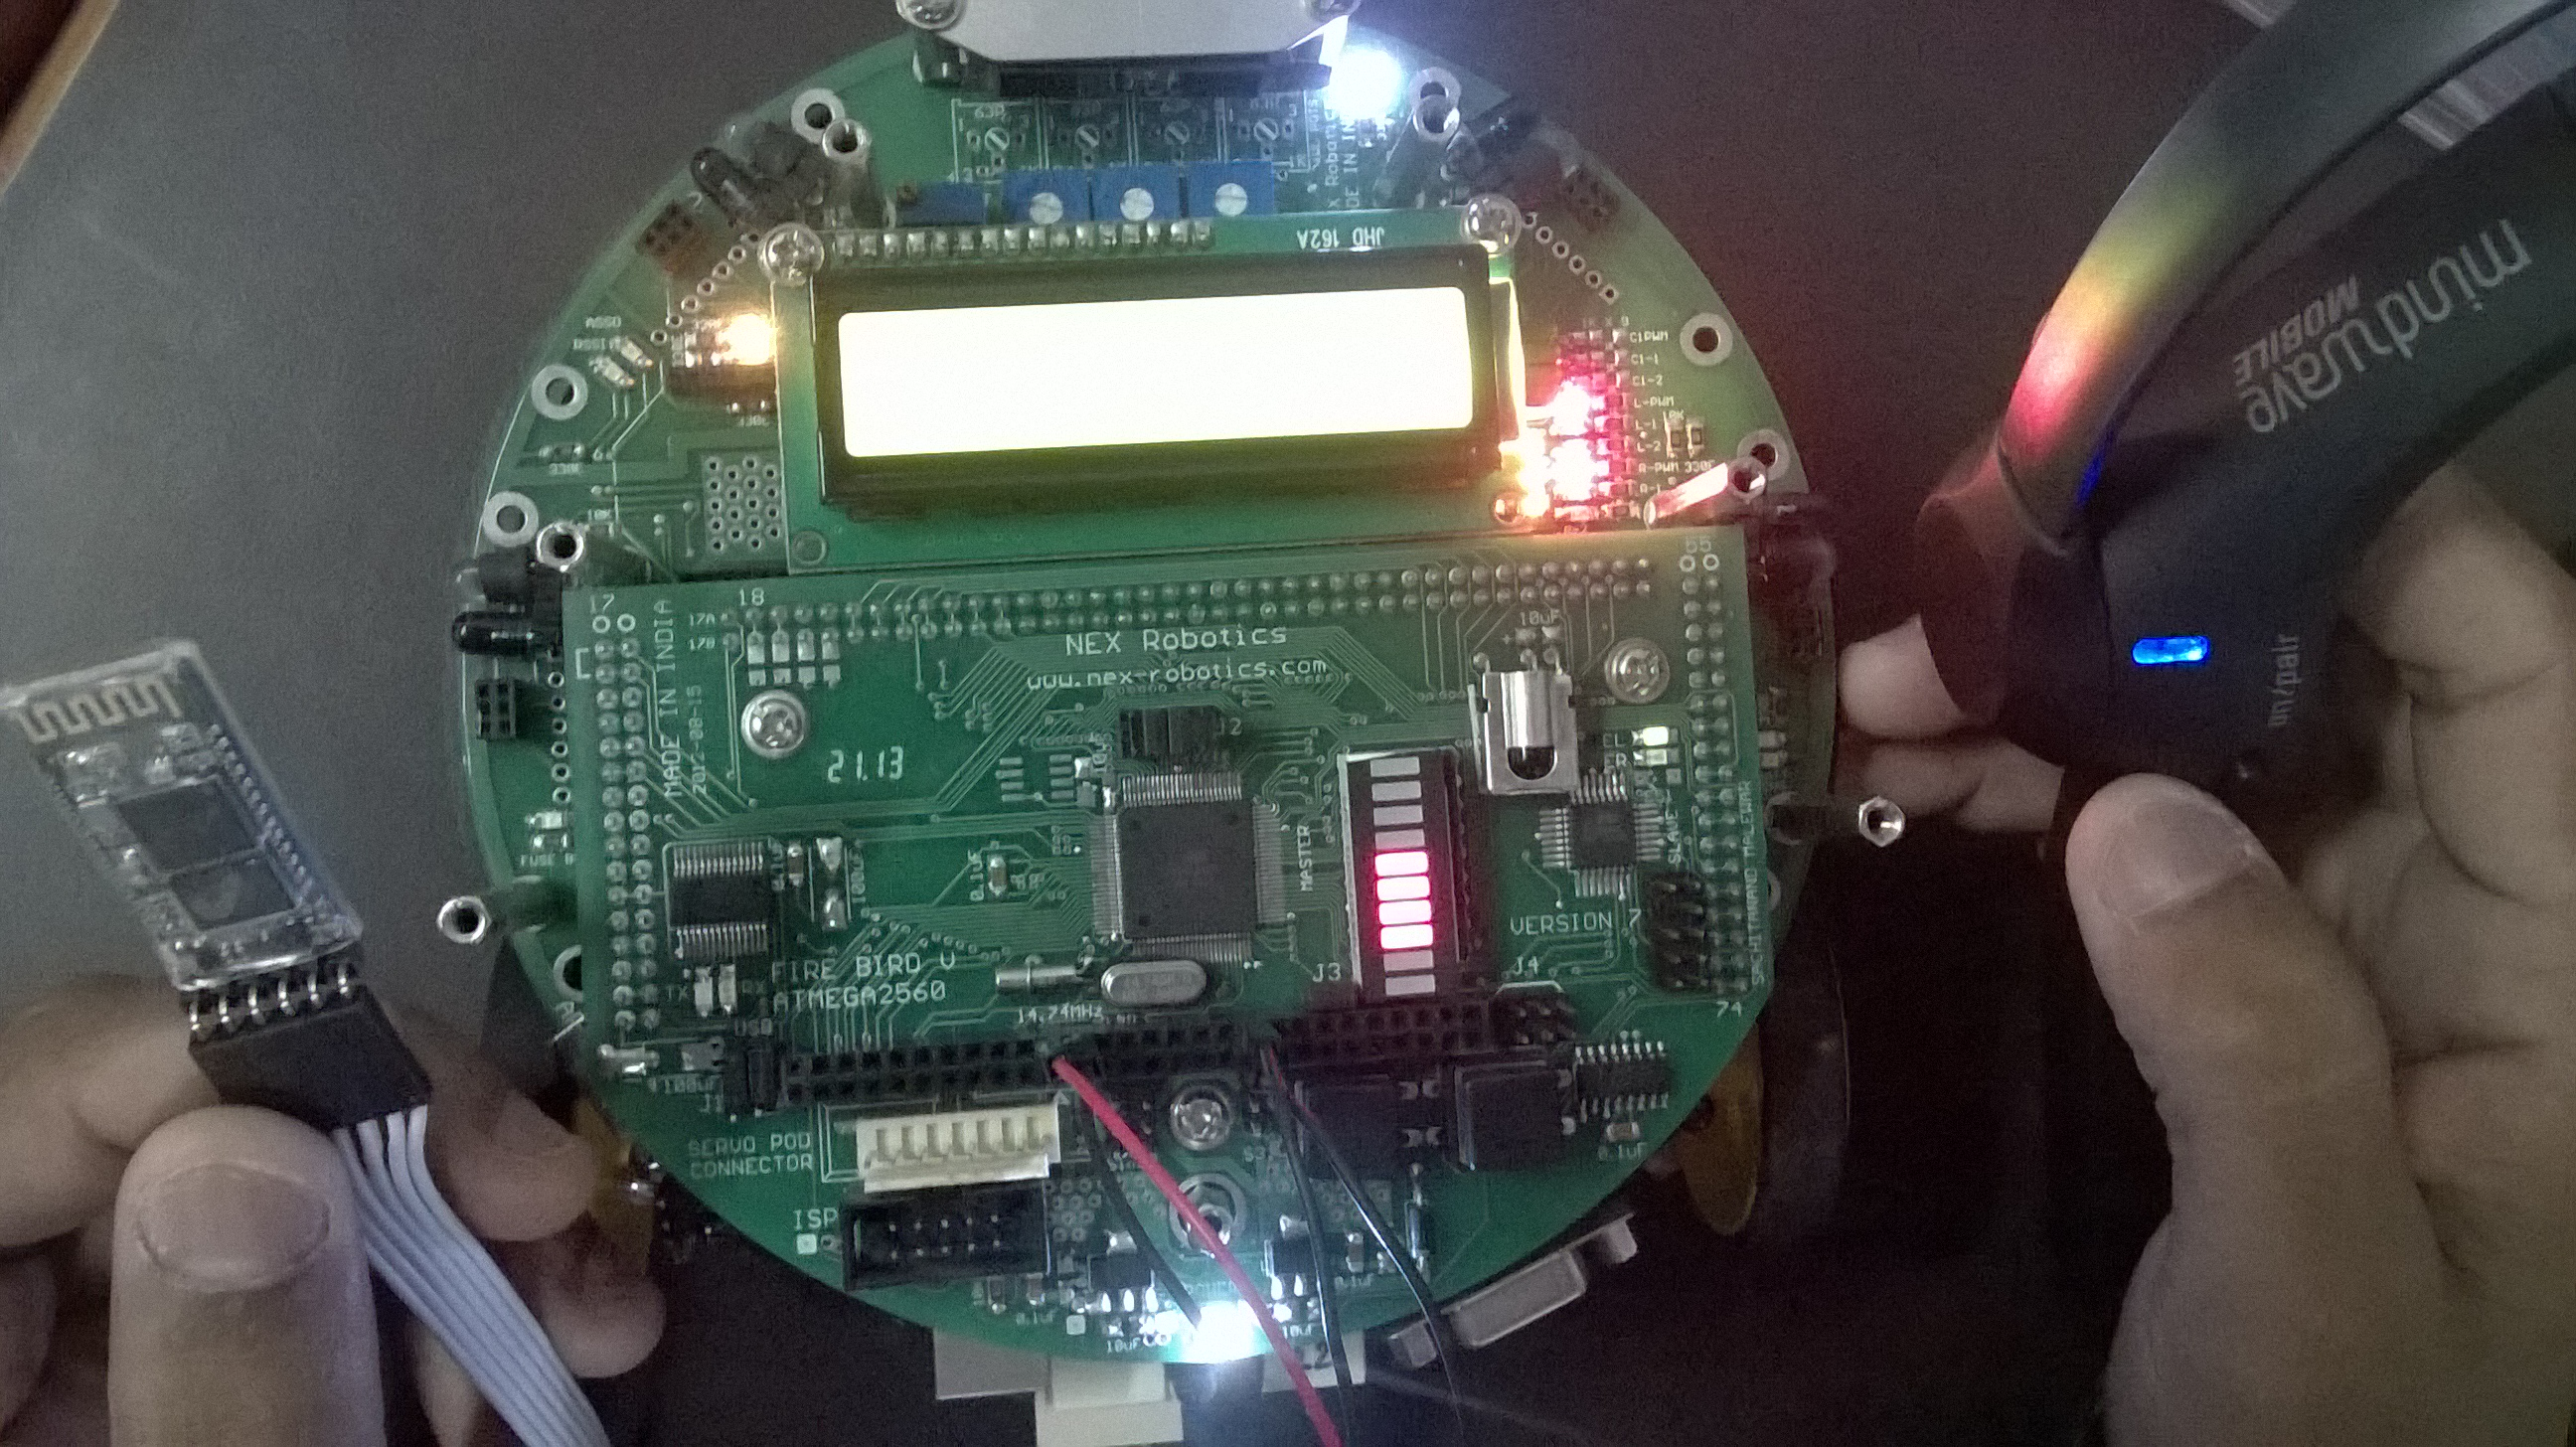
\includegraphics[width=6cm, height=3.2cm]{interfacing}
		\centering
	\end{figure}
\end{itemize}
\end{frame}

\section{Task 4:Attention Level detection}
\begin{frame}{Attention Level Detection}
	\begin{itemize}
		\item Attention level from 1-10 percent indicates mind-wandering event.
		\item Attention level from 10-30 percent indicates poor quality of attention achieved.
		\item Attention level from 40-60 percent indicates neutrality.
		\item Attention level of more than 70 to 80 percent cannot be achieved often.
		
	\end{itemize}
\end{frame}

\section{Challenges Faced}
\begin{frame}{Challenges faced during project}
	\begin{itemize}
		\item Receiving data using bluetooth module.
		\item Receiving a proper data packet from the mindwave sensor.
		\item Processing delay of program compared to time taken to receive continuous data packets.
		\item Detection of random data values during connection of sensor with scalp and during disconnecting it.
		\item Analysing eye-blink data values.   
	\end{itemize}
\end{frame}

\section{Future Plans}
\begin{frame}{Future Plans}
	\begin{itemize}
		\item Analyzing eye-blink data values and increasing accuracy of it.
		\item Controlling Firebird V motions (Right, left, forward, stop) using attention level and eye-blink.
		\item Applying similar technique to control wheel-chair.
	\end{itemize}
\end{frame}


\section{Thank You}
\begin{frame}{Questions are welcome}
	\centering \textbf{THANK YOU !!!}
\end{frame}
\end{document}
